\documentclass{standalone}
\usepackage{tikz}
\usetikzlibrary{patterns, positioning}


\begin{document}
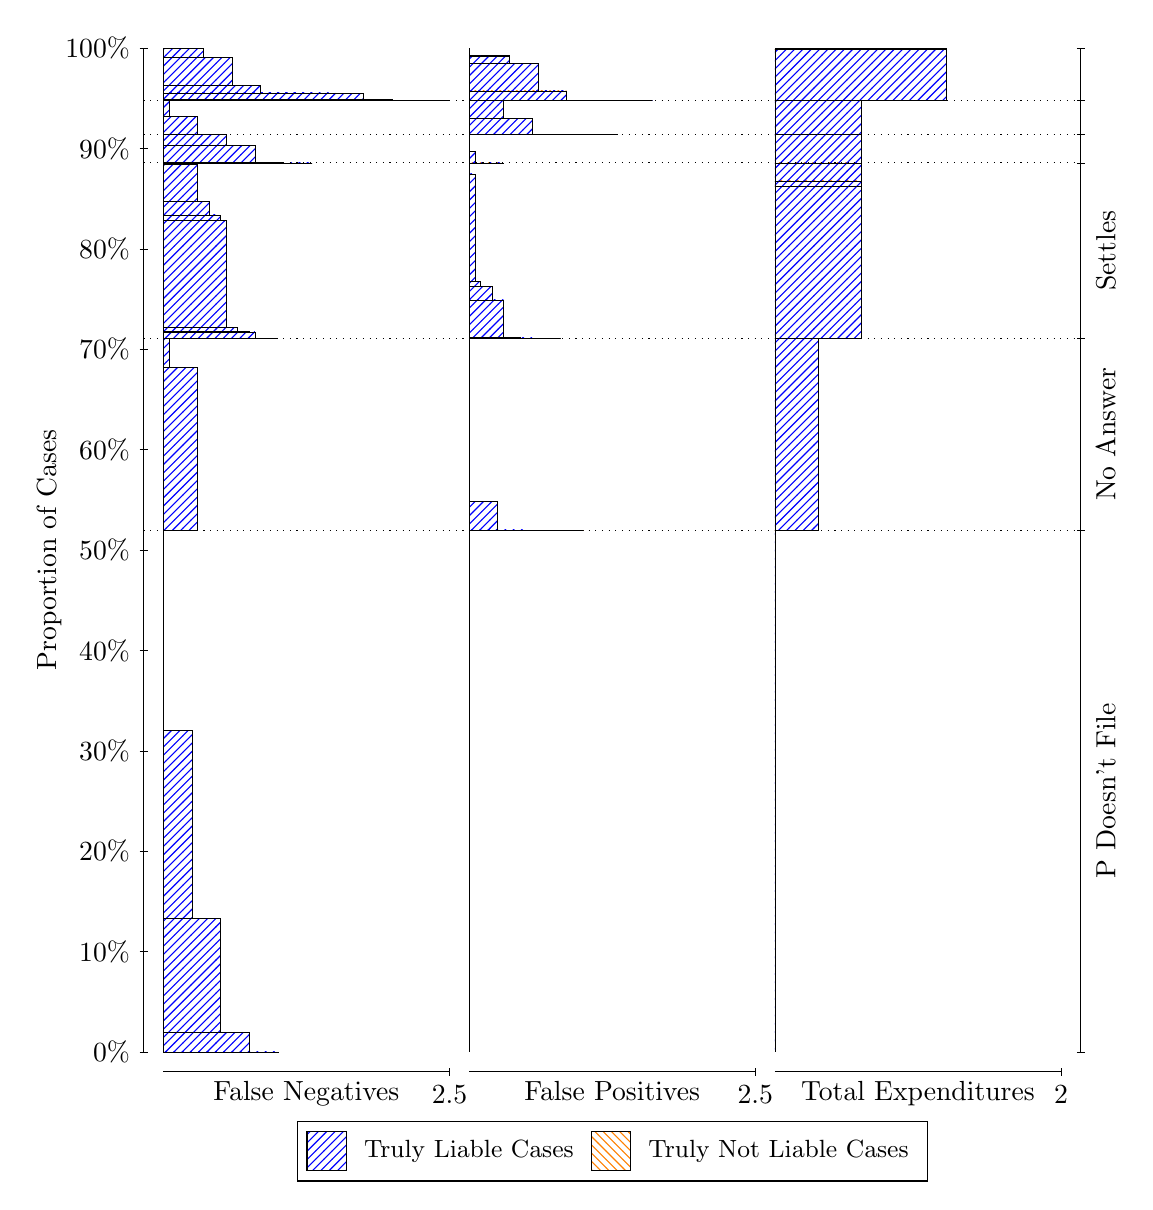
\begin{tikzpicture}
\draw[black, very thin] (1.5,1.75) -- (1.5,14.5);
\node[rotate=90, text=black, anchor=center] at (0.3, 8.125) {Proportion of Cases};
\draw[black, very thin] (1.45,1.75) -- (1.55,1.75);
\node[text=black, anchor=east] at (1.45, 1.75) {0\%};
\draw[black, very thin] (1.45,3.025) -- (1.55,3.025);
\node[text=black, anchor=east] at (1.45, 3.025) {10\%};
\draw[black, very thin] (1.45,4.3) -- (1.55,4.3);
\node[text=black, anchor=east] at (1.45, 4.3) {20\%};
\draw[black, very thin] (1.45,5.575) -- (1.55,5.575);
\node[text=black, anchor=east] at (1.45, 5.575) {30\%};
\draw[black, very thin] (1.45,6.85) -- (1.55,6.85);
\node[text=black, anchor=east] at (1.45, 6.85) {40\%};
\draw[black, very thin] (1.45,8.125) -- (1.55,8.125);
\node[text=black, anchor=east] at (1.45, 8.125) {50\%};
\draw[black, very thin] (1.45,9.4) -- (1.55,9.4);
\node[text=black, anchor=east] at (1.45, 9.4) {60\%};
\draw[black, very thin] (1.45,10.675) -- (1.55,10.675);
\node[text=black, anchor=east] at (1.45, 10.675) {70\%};
\draw[black, very thin] (1.45,11.95) -- (1.55,11.95);
\node[text=black, anchor=east] at (1.45, 11.95) {80\%};
\draw[black, very thin] (1.45,13.225) -- (1.55,13.225);
\node[text=black, anchor=east] at (1.45, 13.225) {90\%};
\draw[black, very thin] (1.45,14.5) -- (1.55,14.5);
\node[text=black, anchor=east] at (1.45, 14.5) {100\%};

\draw[black, very thin] (13.4,1.75) -- (13.4,14.5);
\draw[black, very thin] (13.35,1.75) -- (13.45,1.75);
\node[anchor=west] at (13.35, 1.75) {};
\draw[black, very thin] (13.35,8.3779) -- (13.45,8.3779);
\node[anchor=west] at (13.35, 8.3779) {};
\draw[black, very thin] (13.35,10.81) -- (13.45,10.81);
\node[anchor=west] at (13.35, 10.81) {};
\draw[black, very thin] (13.35,13.041) -- (13.45,13.041);
\node[anchor=west] at (13.35, 13.041) {};
\draw[black, very thin] (13.35,13.402) -- (13.45,13.402);
\node[anchor=west] at (13.35, 13.402) {};
\draw[black, very thin] (13.35,13.834) -- (13.45,13.834);
\node[anchor=west] at (13.35, 13.834) {};
\draw[black, very thin] (13.35,14.5) -- (13.45,14.5);
\node[anchor=west] at (13.35, 14.5) {};

\draw[black, very thin, pattern color=blue, pattern=north east lines] (1.75,1.75) rectangle (3.2033,1.7525);
\draw[black, very thin, pattern color=blue, pattern=north east lines] (1.75,1.7525) rectangle (2.84,1.9965);
\draw[black, very thin, pattern color=blue, pattern=north east lines] (1.75,1.9965) rectangle (2.4767,3.444);
\draw[black, very thin, pattern color=blue, pattern=north east lines] (1.75,3.444) rectangle (2.1133,5.8295);
\draw[black, very thin, pattern color=orange, pattern=north west lines] (1.75,5.8295) rectangle (1.75,5.8295);
\draw[black, very thin, pattern color=blue, pattern=north east lines] (1.75,5.8295) rectangle (1.75,8.3779);
\draw[black, very thin, pattern color=blue, pattern=north east lines] (1.75,8.3779) rectangle (2.186,10.445);
\draw[black, very thin, pattern color=blue, pattern=north east lines] (1.75,10.445) rectangle (1.8227,10.808);
\draw[black, very thin, pattern color=orange, pattern=north west lines] (1.75,10.808) rectangle (1.75,10.808);
\draw[black, very thin, pattern color=blue, pattern=north east lines] (1.75,10.808) rectangle (1.75,10.81);
\draw[black, very thin, pattern color=blue, pattern=north east lines] (1.75,10.81) rectangle (3.2033,10.81);
\draw[black, very thin, pattern color=blue, pattern=north east lines] (1.75,10.81) rectangle (3.058,10.81);
\draw[black, very thin, pattern color=blue, pattern=north east lines] (1.75,10.81) rectangle (2.9127,10.894);
\draw[black, very thin, pattern color=blue, pattern=north east lines] (1.75,10.894) rectangle (2.84,10.898);
\draw[black, very thin, pattern color=blue, pattern=north east lines] (1.75,10.898) rectangle (2.6947,10.949);
\draw[black, very thin, pattern color=blue, pattern=north east lines] (1.75,10.949) rectangle (2.5493,12.312);
\draw[black, very thin, pattern color=blue, pattern=north east lines] (1.75,12.312) rectangle (2.4767,12.38);
\draw[black, very thin, pattern color=blue, pattern=north east lines] (1.75,12.38) rectangle (2.3313,12.549);
\draw[black, very thin, pattern color=blue, pattern=north east lines] (1.75,12.549) rectangle (2.186,13.02);
\draw[black, very thin, pattern color=blue, pattern=north east lines] (1.75,13.02) rectangle (2.1133,13.024);
\draw[black, very thin, pattern color=blue, pattern=north east lines] (1.75,13.024) rectangle (1.968,13.031);
\draw[black, very thin, pattern color=blue, pattern=north east lines] (1.75,13.031) rectangle (1.8227,13.041);
\draw[black, very thin, pattern color=orange, pattern=north west lines] (1.75,13.041) rectangle (1.75,13.041);
\draw[black, very thin, pattern color=blue, pattern=north east lines] (1.75,13.041) rectangle (1.75,13.041);
\draw[black, very thin, pattern color=blue, pattern=north east lines] (1.75,13.041) rectangle (3.6393,13.041);
\draw[black, very thin, pattern color=blue, pattern=north east lines] (1.75,13.041) rectangle (3.276,13.046);
\draw[black, very thin, pattern color=blue, pattern=north east lines] (1.75,13.046) rectangle (2.9127,13.259);
\draw[black, very thin, pattern color=blue, pattern=north east lines] (1.75,13.259) rectangle (2.5493,13.4);
\draw[black, very thin, pattern color=blue, pattern=north east lines] (1.75,13.4) rectangle (2.186,13.402);
\draw[black, very thin, pattern color=orange, pattern=north west lines] (1.75,13.402) rectangle (1.75,13.402);
\draw[black, very thin, pattern color=blue, pattern=north east lines] (1.75,13.402) rectangle (2.186,13.631);
\draw[black, very thin, pattern color=blue, pattern=north east lines] (1.75,13.631) rectangle (1.8227,13.832);
\draw[black, very thin, pattern color=orange, pattern=north west lines] (1.75,13.832) rectangle (1.75,13.832);
\draw[black, very thin, pattern color=blue, pattern=north east lines] (1.75,13.832) rectangle (1.75,13.834);
\draw[black, very thin, pattern color=blue, pattern=north east lines] (1.75,13.834) rectangle (5.3833,13.834);
\draw[black, very thin, pattern color=blue, pattern=north east lines] (1.75,13.834) rectangle (5.02,13.835);
\draw[black, very thin, pattern color=blue, pattern=north east lines] (1.75,13.835) rectangle (4.6567,13.851);
\draw[black, very thin, pattern color=blue, pattern=north east lines] (1.75,13.851) rectangle (4.2933,13.923);
\draw[black, very thin, pattern color=blue, pattern=north east lines] (1.75,13.923) rectangle (3.93,13.93);
\draw[black, very thin, pattern color=blue, pattern=north east lines] (1.75,13.93) rectangle (3.712,13.93);
\draw[black, very thin, pattern color=blue, pattern=north east lines] (1.75,13.93) rectangle (3.5667,13.93);
\draw[black, very thin, pattern color=blue, pattern=north east lines] (1.75,13.93) rectangle (3.3487,13.93);
\draw[black, very thin, pattern color=blue, pattern=north east lines] (1.75,13.93) rectangle (3.2033,13.93);
\draw[black, very thin, pattern color=blue, pattern=north east lines] (1.75,13.93) rectangle (2.9853,14.025);
\draw[black, very thin, pattern color=blue, pattern=north east lines] (1.75,14.025) rectangle (2.622,14.38);
\draw[black, very thin, pattern color=blue, pattern=north east lines] (1.75,14.38) rectangle (2.2587,14.496);
\draw[black, very thin, pattern color=blue, pattern=north east lines] (1.75,14.496) rectangle (1.8953,14.5);
\draw[black, very thin, pattern color=orange, pattern=north west lines] (1.75,14.5) rectangle (1.75,14.5);
\draw[black, very thin, pattern color=blue, pattern=north east lines] (1.75,14.5) rectangle (1.75,14.5);
\draw[black, very thin, pattern color=orange, pattern=north west lines] (5.6333,1.75) rectangle (5.6333,1.75);
\draw[black, very thin, pattern color=blue, pattern=north east lines] (5.6333,1.75) rectangle (5.6333,8.3779);
\draw[black, very thin, pattern color=orange, pattern=north west lines] (5.6333,8.3779) rectangle (7.0867,8.3779);
\draw[black, very thin, pattern color=blue, pattern=north east lines] (5.6333,8.3779) rectangle (7.0867,8.3779);
\draw[black, very thin, pattern color=blue, pattern=north east lines] (5.6333,8.3779) rectangle (6.7233,8.3779);
\draw[black, very thin, pattern color=blue, pattern=north east lines] (5.6333,8.3779) rectangle (6.36,8.3794);
\draw[black, very thin, pattern color=blue, pattern=north east lines] (5.6333,8.3794) rectangle (5.9967,8.7426);
\draw[black, very thin, pattern color=blue, pattern=north east lines] (5.6333,8.7426) rectangle (5.6333,10.81);
\draw[black, very thin, pattern color=orange, pattern=north west lines] (5.6333,10.81) rectangle (6.796,10.81);
\draw[black, very thin, pattern color=blue, pattern=north east lines] (5.6333,10.81) rectangle (6.796,10.81);
\draw[black, very thin, pattern color=orange, pattern=north west lines] (5.6333,10.81) rectangle (6.6507,10.81);
\draw[black, very thin, pattern color=blue, pattern=north east lines] (5.6333,10.81) rectangle (6.6507,10.81);
\draw[black, very thin, pattern color=orange, pattern=north west lines] (5.6333,10.81) rectangle (6.5053,10.81);
\draw[black, very thin, pattern color=blue, pattern=north east lines] (5.6333,10.81) rectangle (6.5053,10.81);
\draw[black, very thin, pattern color=blue, pattern=north east lines] (5.6333,10.81) rectangle (6.4327,10.82);
\draw[black, very thin, pattern color=blue, pattern=north east lines] (5.6333,10.82) rectangle (6.2873,10.827);
\draw[black, very thin, pattern color=blue, pattern=north east lines] (5.6333,10.827) rectangle (6.142,10.83);
\draw[black, very thin, pattern color=blue, pattern=north east lines] (5.6333,10.83) rectangle (6.0693,11.301);
\draw[black, very thin, pattern color=blue, pattern=north east lines] (5.6333,11.301) rectangle (5.924,11.47);
\draw[black, very thin, pattern color=blue, pattern=north east lines] (5.6333,11.47) rectangle (5.7787,11.539);
\draw[black, very thin, pattern color=blue, pattern=north east lines] (5.6333,11.539) rectangle (5.706,12.901);
\draw[black, very thin, pattern color=blue, pattern=north east lines] (5.6333,12.901) rectangle (5.6333,13.041);
\draw[black, very thin, pattern color=orange, pattern=north west lines] (5.6333,13.041) rectangle (6.0693,13.041);
\draw[black, very thin, pattern color=blue, pattern=north east lines] (5.6333,13.041) rectangle (6.0693,13.042);
\draw[black, very thin, pattern color=blue, pattern=north east lines] (5.6333,13.042) rectangle (5.706,13.183);
\draw[black, very thin, pattern color=blue, pattern=north east lines] (5.6333,13.183) rectangle (5.6333,13.402);
\draw[black, very thin, pattern color=orange, pattern=north west lines] (5.6333,13.402) rectangle (7.5227,13.402);
\draw[black, very thin, pattern color=blue, pattern=north east lines] (5.6333,13.402) rectangle (7.5227,13.402);
\draw[black, very thin, pattern color=blue, pattern=north east lines] (5.6333,13.402) rectangle (7.1593,13.402);
\draw[black, very thin, pattern color=blue, pattern=north east lines] (5.6333,13.402) rectangle (6.796,13.404);
\draw[black, very thin, pattern color=blue, pattern=north east lines] (5.6333,13.404) rectangle (6.4327,13.606);
\draw[black, very thin, pattern color=blue, pattern=north east lines] (5.6333,13.606) rectangle (6.0693,13.834);
\draw[black, very thin, pattern color=orange, pattern=north west lines] (5.6333,13.834) rectangle (7.9587,13.834);
\draw[black, very thin, pattern color=blue, pattern=north east lines] (5.6333,13.834) rectangle (7.9587,13.834);
\draw[black, very thin, pattern color=orange, pattern=north west lines] (5.6333,13.834) rectangle (7.5953,13.834);
\draw[black, very thin, pattern color=blue, pattern=north east lines] (5.6333,13.834) rectangle (7.5953,13.834);
\draw[black, very thin, pattern color=orange, pattern=north west lines] (5.6333,13.834) rectangle (7.232,13.834);
\draw[black, very thin, pattern color=blue, pattern=north east lines] (5.6333,13.834) rectangle (7.232,13.838);
\draw[black, very thin, pattern color=blue, pattern=north east lines] (5.6333,13.838) rectangle (6.8687,13.955);
\draw[black, very thin, pattern color=orange, pattern=north west lines] (5.6333,13.955) rectangle (6.8687,13.955);
\draw[black, very thin, pattern color=blue, pattern=north east lines] (5.6333,13.955) rectangle (6.8687,13.955);
\draw[black, very thin, pattern color=blue, pattern=north east lines] (5.6333,13.955) rectangle (6.5053,14.308);
\draw[black, very thin, pattern color=blue, pattern=north east lines] (5.6333,14.308) rectangle (6.5053,14.309);
\draw[black, very thin, pattern color=blue, pattern=north east lines] (5.6333,14.309) rectangle (6.142,14.39);
\draw[black, very thin, pattern color=blue, pattern=north east lines] (5.6333,14.39) rectangle (6.142,14.405);
\draw[black, very thin, pattern color=orange, pattern=north west lines] (5.6333,14.405) rectangle (5.924,14.405);
\draw[black, very thin, pattern color=blue, pattern=north east lines] (5.6333,14.405) rectangle (5.924,14.405);
\draw[black, very thin, pattern color=blue, pattern=north east lines] (5.6333,14.405) rectangle (5.7787,14.405);
\draw[black, very thin, pattern color=blue, pattern=north east lines] (5.6333,14.405) rectangle (5.7787,14.405);
\draw[black, very thin, pattern color=orange, pattern=north west lines] (5.6333,14.405) rectangle (5.6333,14.405);
\draw[black, very thin, pattern color=blue, pattern=north east lines] (5.6333,14.405) rectangle (5.6333,14.5);
\draw[black, very thin, pattern color=orange, pattern=north west lines] (9.5167,1.75) rectangle (9.5167,1.75);
\draw[black, very thin, pattern color=blue, pattern=north east lines] (9.5167,1.75) rectangle (9.5167,8.3779);
\draw[black, very thin, pattern color=orange, pattern=north west lines] (9.5167,8.3779) rectangle (10.062,8.3779);
\draw[black, very thin, pattern color=blue, pattern=north east lines] (9.5167,8.3779) rectangle (10.062,10.81);
\draw[black, very thin, pattern color=orange, pattern=north west lines] (9.5167,10.81) rectangle (10.607,10.81);
\draw[black, very thin, pattern color=blue, pattern=north east lines] (9.5167,10.81) rectangle (10.607,12.738);
\draw[black, very thin, pattern color=orange, pattern=north west lines] (9.5167,12.738) rectangle (10.607,12.738);
\draw[black, very thin, pattern color=blue, pattern=north east lines] (9.5167,12.738) rectangle (10.607,12.813);
\draw[black, very thin, pattern color=orange, pattern=north west lines] (9.5167,12.813) rectangle (10.607,12.813);
\draw[black, very thin, pattern color=blue, pattern=north east lines] (9.5167,12.813) rectangle (10.607,13.041);
\draw[black, very thin, pattern color=orange, pattern=north west lines] (9.5167,13.041) rectangle (10.607,13.041);
\draw[black, very thin, pattern color=blue, pattern=north east lines] (9.5167,13.041) rectangle (10.607,13.402);
\draw[black, very thin, pattern color=orange, pattern=north west lines] (9.5167,13.402) rectangle (10.607,13.402);
\draw[black, very thin, pattern color=blue, pattern=north east lines] (9.5167,13.402) rectangle (10.607,13.834);
\draw[black, very thin, pattern color=orange, pattern=north west lines] (9.5167,13.834) rectangle (11.697,13.834);
\draw[black, very thin, pattern color=blue, pattern=north east lines] (9.5167,13.834) rectangle (11.697,14.483);
\draw[black, very thin, pattern color=orange, pattern=north west lines] (9.5167,14.483) rectangle (11.697,14.483);
\draw[black, very thin, pattern color=blue, pattern=north east lines] (9.5167,14.483) rectangle (11.697,14.5);
\draw[black, dotted] (1.5,8.3779) -- (13.4,8.3779);
\draw[black, dotted] (1.5,10.81) -- (13.4,10.81);
\draw[black, dotted] (1.5,13.041) -- (13.4,13.041);
\draw[black, dotted] (1.5,13.402) -- (13.4,13.402);
\draw[black, dotted] (1.5,13.834) -- (13.4,13.834);
\draw[black, very thin] (1.75,1.5) -- (5.3833,1.5);
\node[text=black, anchor=north] at (3.5667, 1.5) {False Negatives};
\draw[black, very thin] (5.3833,1.45) -- (5.3833,1.55);
\node[text=black, anchor=north] at (5.3833, 1.45) {2.5};

\draw[black, very thin] (5.6333,1.5) -- (9.2667,1.5);
\node[text=black, anchor=north] at (7.45, 1.5) {False Positives};
\draw[black, very thin] (9.2667,1.45) -- (9.2667,1.55);
\node[text=black, anchor=north] at (9.2667, 1.45) {2.5};

\draw[black, very thin] (9.5167,1.5) -- (13.15,1.5);
\node[text=black, anchor=north] at (11.333, 1.5) {Total Expenditures};
\draw[black, very thin] (13.15,1.45) -- (13.15,1.55);
\node[text=black, anchor=north] at (13.15, 1.45) {2};

\node[text=black, centered, rotate=90] at (13.72, 5.0639) {P Doesn't File};
\node[text=black, centered, rotate=90] at (13.72, 9.5938) {No Answer};
\node[text=black, centered, rotate=90] at (13.72, 11.925) {Settles};




\draw (7.449999999999999,1.5) node[draw=none] (baseCoordinate) {};
\begin{scope}[align=center]
        \matrix[scale=0.5, draw=black, below=0.5cm of baseCoordinate, nodes={draw}, column sep=0.1cm]{
            \node[rectangle, draw, minimum width=0.5cm, minimum height=0.5cm, pattern color=blue, pattern=north east lines] {}; &
            \node[draw=none, font=\small, text=black] (B) {Truly Liable Cases}; &
            \node[rectangle, draw, minimum width=0.5cm, minimum height=0.5cm, pattern color=orange, pattern=north west lines] {}; &
            \node[draw=none, font=\small, text=black] (B) {Truly Not Liable Cases}; \\
            };
\end{scope}

\end{tikzpicture}
\end{document}